\documentclass[11pt, a4paper, twocolumn]{article}

%%%%%%%%%%%%%%%%%
% Configuration %
%%%%%%%%%%%%%%%%%
\usepackage{allrunes}
\usepackage{amsmath}
% If magyar is wanted
%\usepackage[magyar]{babel}

\usepackage[T1]{fontenc}
\usepackage[utf8]{inputenc}
\usepackage{fixltx2e}
\usepackage{multirow}
\usepackage{url}
\usepackage{amsfonts}
\usepackage{amsthm}
\usepackage{amssymb}

\newcommand{\abstractText}{\noindent
  Abstract goes here.
}

% Here you can configure the layout
\usepackage{geometry}
\geometry{top=1cm, bottom=1cm, left=1.25cm,right=1.25cm, includehead, includefoot}
\setlength{\columnsep}{7mm} % Column separation width

\usepackage{graphicx}

%\usepackage{gensymb}
\usepackage{float}

% For bra-ket notation
\usepackage{braket}

% To have a good appendix
\usepackage[toc,page]{appendix}

\usepackage{abstract}
\renewcommand{\abstractnamefont}{\normalfont\bfseries}
\renewcommand{\abstracttextfont}{\normalfont\small\itshape}
\usepackage{lipsum}

%%%%%%%%%%%%%%%%%%%
% Custom commands %
%%%%%%%%%%%%%%%%%%%
\newcommand{\bb}[1]{\mathbf{#1}}


% Hyperref should be generally the last package to load
% Any configuration that should be done before the end of the preamble:
\usepackage{hyperref}
\hypersetup{colorlinks=true, urlcolor=blue, linkcolor=blue, citecolor=blue}

\title{Numerical simulation of quantum transport phenomena}

\author{Nagy Dániel}

\begin{document}

%%%%%%%%%%%%
% Abstract %
%%%%%%%%%%%%

\twocolumn[
  \begin{@twocolumnfalse}
    \maketitle
    \begin{abstract}
      In recent years electronic transport properties of a variety of low dimensional electron systems,
    such as carbon based novel materials like carbon nanotubes or graphene, boron nitride, dichalcogenides, 
    a selection of intriguing molecules and the surface states of topological insulators has captured the imagination of the 
    solid-state community. These systems have several interesting properties that make them not only interesting for theoretical 
    investigations but could also lead to revolutionary applications from wearable electronics to quantum computers. 
    To take control of these peculiar features a comprehensive and detailed theoretical study is needed. 
    During my work, I used Kwant to investigate these systems by numerical calculations. Kwant is a free and open source, 
    powerful, and easy to use Python package for numericalccalculations on tight-binding models with 
    a strong focus on quantum transport.
      \newline
      \newline
    \end{abstract}
  \end{@twocolumnfalse}
]

%%%%%%%%%%%
% Article %
%%%%%%%%%%%

\section*{Introduction}

\section*{The tight binding approximation}
One of the main goals of solid-state physics is to explain phyisical properties of crystals,
such as band structure, conductance, etc. based on their geometry. The energy eigenstates of 
an electron can be found by solving the stationary Scröinger equation:
\begin{equation*}
  \left[ -\frac{\hbar^2}{2m} \nabla^2 + V(\bb r) \right]\Psi_n(\bb r) = E_n\Psi_n(\bb r)
\end{equation*}
Solving this equation is very hard in general, but thanks to the lattice-periodic structure of crystals,
several approximate calculations can be made. One of these approximations is the so-called tight binding approximation,
which is often used in solid-state physics. 
\par The tight binding approximation assumes, that electrons are tightly bound to atoms to which they belong, and the effect 
of the other atoms arises as a perturbation.

First denote $\hat H_{\textrm{at}}$ the Hamiltonian of a single, isolated atom, and its eigenfunctions $\varphi_{\alpha}(\bb r)$.
Here, $\alpha$ represents all the internal degrees of freedom e.g. spin, atomic orbital, etc.
These functions are solutions to the single-atom Schrödinger-equation
\begin{equation*}
  \underbrace{ \left[ -\frac{\hbar^2}{2m} \nabla^2 + V_{\textrm{at}}(\bb r) \right]}_{\hat H_{\textrm{at}}} \varphi_{\alpha}(\bb r)
  = \varepsilon_{\alpha}\varphi_{\alpha}({\bb r})~\textrm{, }
\end{equation*}

The full Hamiltonian can be written as
\begin{equation*}
  \hat H = -\frac{\hbar^2}{2m} \nabla^2 + \sum\limits_{\bb{R}_n} V_{\textrm{at}} (\bb r - \bb{R}_n)
\end{equation*}
where $\bb{R}_n$ are vectors pointing to the atoms in the lattice.

The idea is to write $\ket\Psi = \Psi(\bb r)$ as a linear combination of atomic wavefunctions localized to the neigboring atoms.
Denoting with $\ket n = \varphi_{n, \alpha}(\bb r)$ the atomic wavefunction localized to the ion at $\bb{R}_n$, $\ket\Psi$ can be
written as:
\begin{equation*}
  \ket\Psi = \sum\limits_{n} b_n \ket n
\end{equation*}
which is written back to the full Schrödinger-equation:
\begin{equation*}
  \sum\limits_n b_n \hat H \ket n = E \sum\limits_n b_n \ket n
\end{equation*}
To be able to numerically solve this eigenvalue-problem, we need to calculate the matrix elements of the 
Hamiltonian:
\begin{equation*}
  \sum\limits_n b_n \braket{m | \hat H | n} = E \sum\limits_n b_n \braket{m|n}
\end{equation*}
In the nearest-neighbor approximation, only the first neighbors are taken into consideration, all other matrix elements
are neglected.
In this case, 
\begin{equation*}
  H_{nn} = \braket{n|\hat H|n} = E_0 \textrm{, and}
\end{equation*}
\begin{equation*}
  H_{mn} = \braket{m|\hat H|n} = -\gamma \textrm{, if $m$ and $n$ are neighbors.}
\end{equation*}

$E_0$ is the \textit{on-site energy} and is not equal to the atomic energy level, due to the perturbation of the neigboring
electrons. $\gamma$ is an empirical parameter and is called the \textit{hopping amplitude}.

% The second ecuation is due to the translational symmetry of the system:$\braket{n-1|\hat H|n} = \braket{n|\hat H|n+1}
% = \braket{n+1|\hat H|n}^{*}$
% \begin{figure}[h!]
%     \begin{center}
%     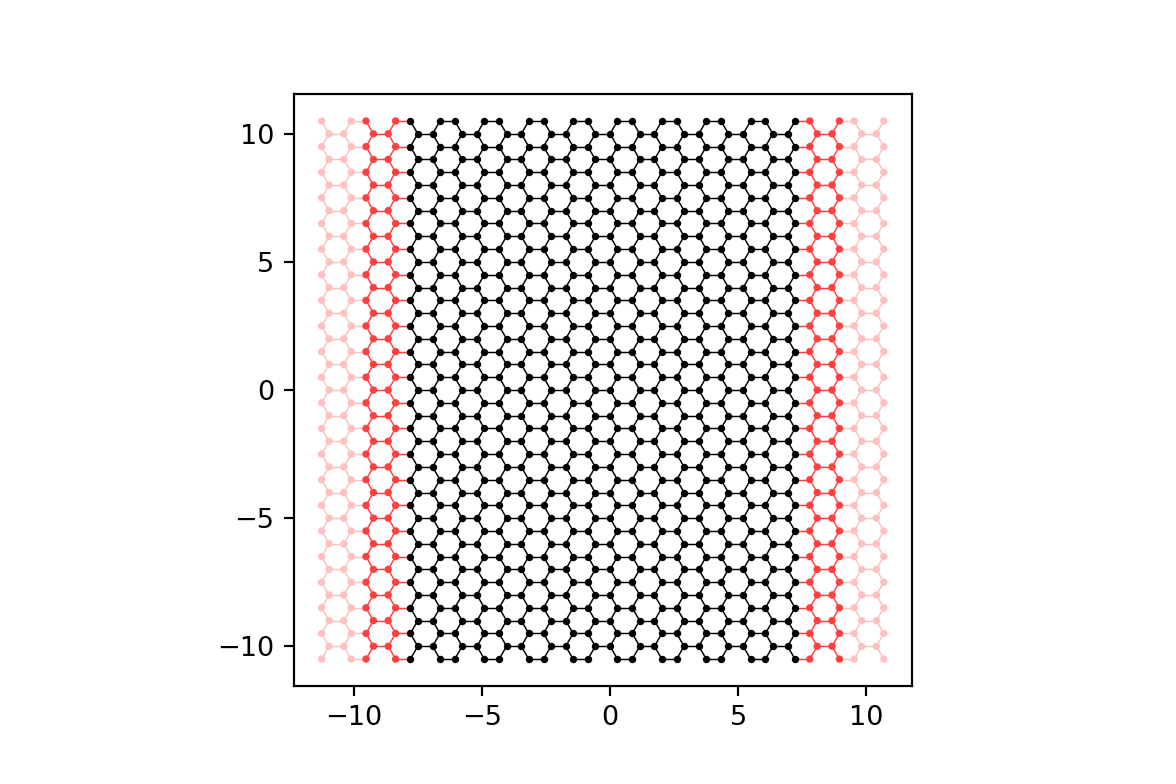
\includegraphics[width=0.45\textwidth]{./media/img1.png}
%     \caption{Some figure}
%     \label{fig:fig1}
%     \end{center}
% \end{figure}

%%%%%%%%%%%%%%
% References %
%%%%%%%%%%%%%%

\nocite{*}
\bibliographystyle{plain}
\bibliography{references}

%%%%%%%%%%%%%%
% Appendices %
%%%%%%%%%%%%%%
\appendix
\section{Some appendix}
\subsection{Some subsection}
\lipsum[6]
\lipsum[7]

% \begin{figure}[htb]
%     \begin{minipage}[t]{.49\textwidth}
%         \centering
%         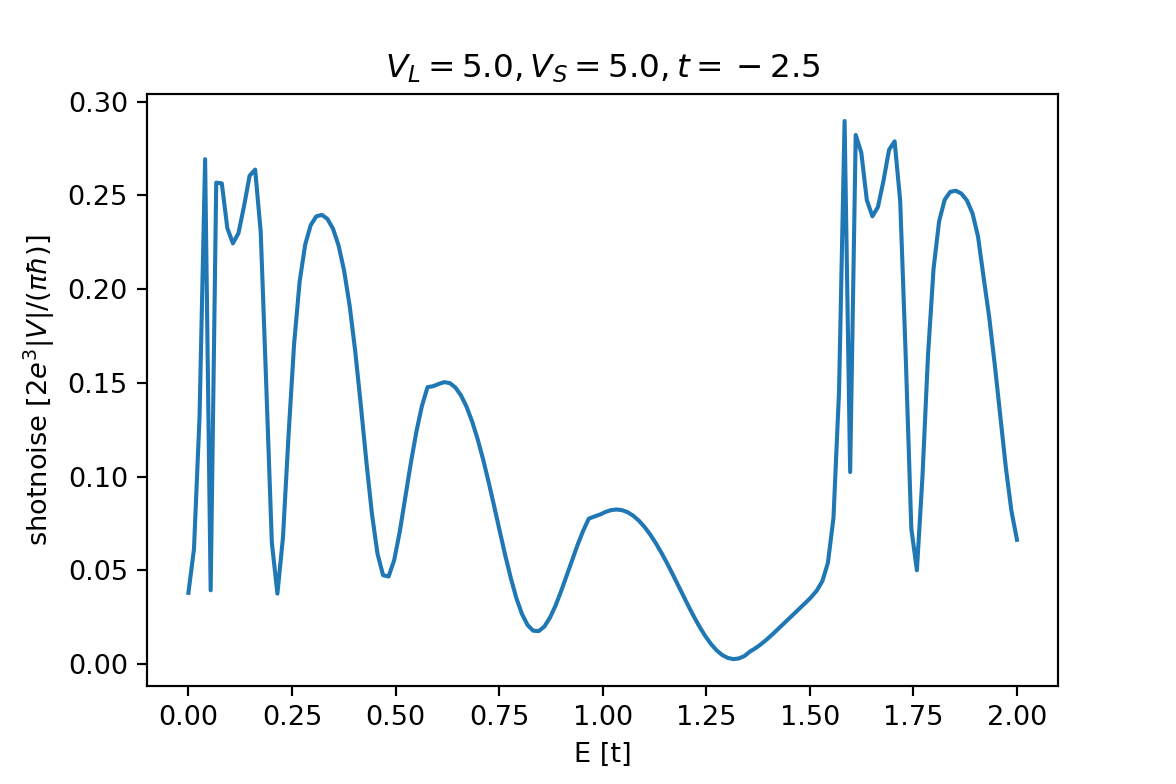
\includegraphics[width=\textwidth]{./media/img2.png}
%         \caption{Image 2}\label{fig:fig2}
%     \end{minipage}
%     \hfill
%     \begin{minipage}[t]{.49\textwidth}
%         \centering
%         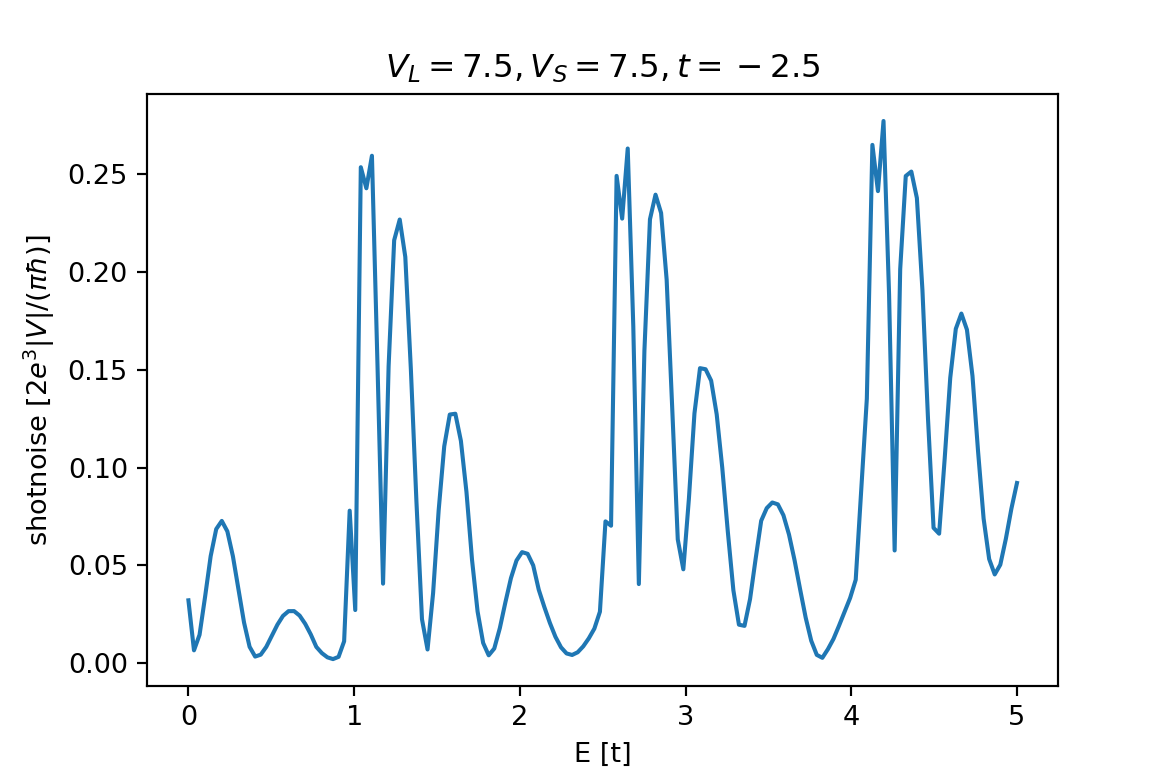
\includegraphics[width=\textwidth]{./media/img3.png}
%         \caption{Image 3}\label{fig:fig3}
%     \end{minipage}
% \end{figure}

\lipsum[8]
\lipsum[9]


\end{document}

